\section{Introduction}
% problem description: semantic relatedness
Computing semantic relatedness(SR) between two elements is a fundamental 
task for many applications in Natural Language Processing(NLP) such as 
word sense disambiguation(\cite{}), information retrieval(\cite{}), 
interpretation of noun compounds and spelling correction.  In this paper 
we focus on computing semantic relatedness between two words in knowledge 
graph with neural network.

It has long been thought that when human measure the relatedness between 
a pair of words, a deeper reasoning is triggered to compare the concepts 
behind the words. There are so many data sources offer various knowledge 
hidden behind the words. While many traditional studies on semantic relatedness 
utilize the lexical databases, such as WordNet or Wikitionary\cite{}, (!!!)
the recent word embedding learning approaches demonstrate their abilities 
to capture syntactic and semantic information, and outperform the 
lexicon-based methods\cite{}. Knowledge Graph, as a semantic graph, stores
vast amount of sturctured knowledge. As a wealth of knowledge, knowledge 
graph can be accessed with regard to the way of storage such as Cypher
in Neo4j(graph database) and Sparql for RDF storage.

% 缺少说明原始方法需要大量的预处理的问题。
Some researchs have attached importance to measure semantic relatedness
in knowledge graph\cite{REWORD, SenseEmbed} recently. Trajep\cite{SenseEmbed} 
leverage entity linking to annotate the dump of wikipedia. Based on this, 
the sense-annotated corpus is generated. Then the author using word2vec to 
train the sense-annotated corpus. this step still need a significant 
preprocessing and data transformation effort. As we can see the author 
just put the knowledge graph on the position of backup. Trajep \cite{REWORD}
propose an approache exploiting the graph nature of RDF and SPARQL query
Language to access knowledge graph. It not only obtains the comparable
result with the state-of-art at that moment, but also avoids the burden 
of preprocessing and data transformation. 

\begin{figure*}
    \centering
    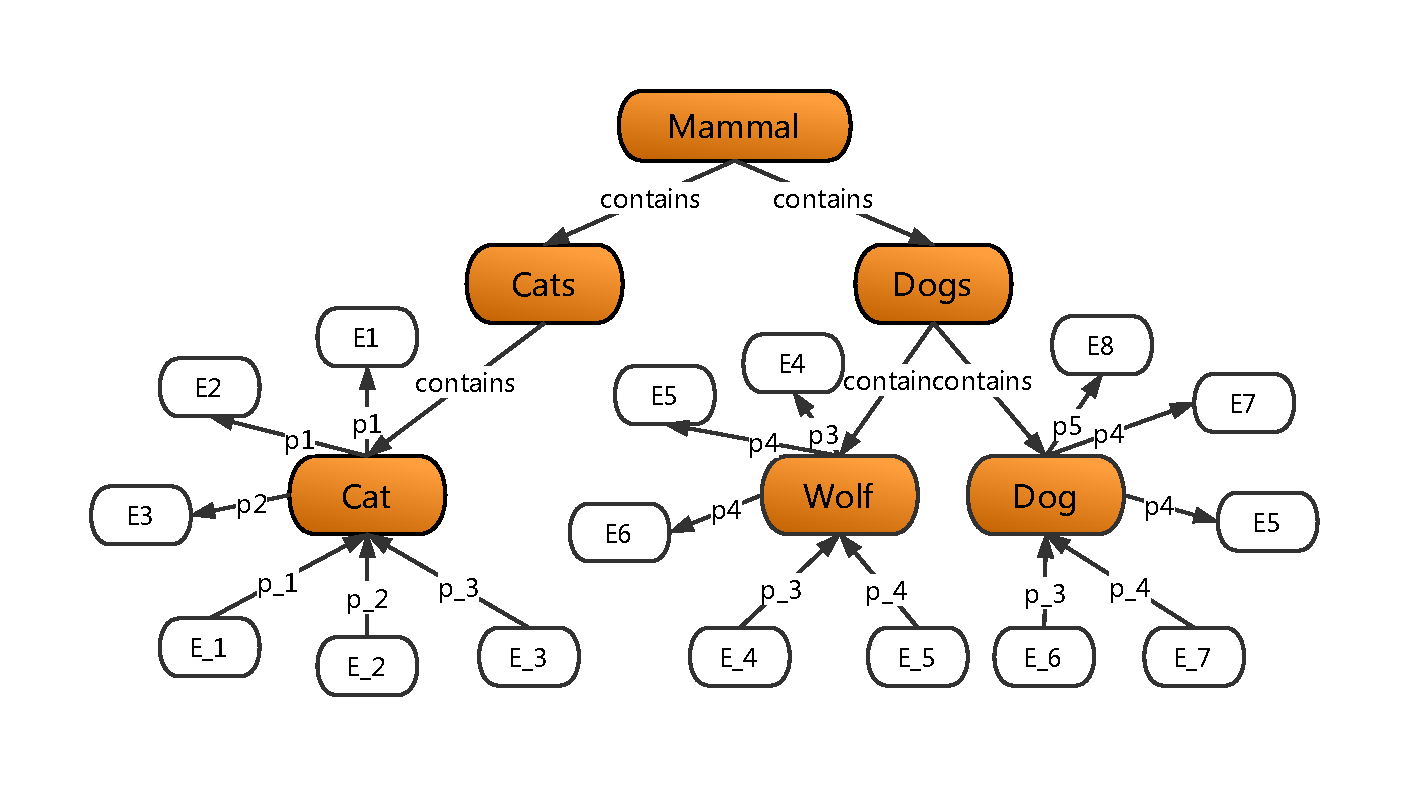
\includegraphics[width=1.0\textwidth]{pic/weak1.pdf}\\
    \caption{Subgraph example in knowledge graph}
    \label{weak1}
\end{figure*}


Though Trajep \cite{REWOED} avoids a significant preprocessing and data
transformation effort, which develops it scalability when adopting a
different source of knowledge graph, they miss some factors which 
have contributed to semantic relatedness measure. Firstly, given two words
as input, the first step is to find corresponding entities in knowledge
graph. Obviously, there are not only one entity in knowledge graph for a single
word. For a input word \emph{car}, for example, we will get \emph{:Automobile} and 
\emph{:Auto\underline{\hspace{0.5em}}Racing} and so on. Trajep lose
sight of the informativeness of the other entities, while they just
consider the entity with the highest rank. Secondly, Trajep misses
some informativeness of \emph{predicates} as their stategy takes
the predicates into account exclusively based on the TFIDF. This 
method ignore the function of \emph{objects} in a semantic triple. 
As show in Fig\ref{weak1}, we 

% knowledge graph
Computing semantic relatedness(SR) between two elements is a fundamental 
task for many applications in Natural Language Processing(NLP) such as 
word sense disambiguation(\cite{}), information retrieval(\cite{}), 
interpretation of noun compounds and spelling correction. Many researchers
confound the defination of semantic relatedness with sematnic similarity.
Strictly, semantic relatedness is a more general concept than semantic 
similarity as it captures not only closeness between two elements within
a type hierarchy(e.g., river and stream), but also any other relations
(e.g., river and boat)(\cite{BudanitskyH06}). As a result, computational
applications typically require relatedness rather than just similarity.

% our contribution
Computing semantic relatedness(SR) between two elements is a fundamental 
task for many applications in Natural Language Processing(NLP) such as 
word sense disambiguation(\cite{}), information retrieval(\cite{}), 
interpretation of noun compounds and spelling correction. Many researchers
confound the defination of semantic relatedness with sematnic similarity.
Strictly, semantic relatedness is a more general concept than semantic 
similarity as it captures not only closeness between two elements within
a type hierarchy(e.g., river and stream), but also any other relations
(e.g., river and boat)(\cite{BudanitskyH06}). As a result, computational
applications typically require relatedness rather than just similarity.

% conclusion
Computing semantic relatedness(SR) between two elements is a fundamental 
task for many applications in Natural Language Processing(NLP) such as 
word sense disambiguation(\cite{}), information retrieval(\cite{}), 
interpretation of noun compounds and spelling correction. Many researchers
confound the defination of semantic relatedness with sematnic similarity.
Strictly, semantic relatedness is a more general concept than semantic 
similarity as it captures not only closeness between two elements within
a type hierarchy(e.g., river and stream), but also any other relations
(e.g., river and boat)(\cite{BudanitskyH06}). As a result, computational
applications typically require relatedness rather than just similarity.